\documentclass[12pt,letterpaper]{article}
\usepackage{preamble}
\usepackage{graphicx}
\usepackage{subcaption}

%%%%%%%%%%%%%%%%%%%%%%%%%%%%%%%%%%%%%%%%%%
%%%% Edit These for yourself
%%%%%%%%%%%%%%%%%%%%%%%%%%%%%%%%%%%%%%%%%%
\newcommand\course{}
\newcommand\hwnumber{1}
\newcommand\userID{Marina E. Almenzar}

\begin{document}
\section*{Programming Exercise 2}
\subsection*{Decision Trees}
Partition the dataset into a training and a testing set.
Run a decision tree learning algorithm using the training set. Test the
decision tree on the testing dataset and report the total classification error
(i.e. 0/1 error). Repeat the experiment with a different partition. Plot
the resulting trees. Are they very similar, or very different? Explain why.

Advice: it can be convenient to set a maximum depth for the tree.
\begin{figure}[H]
    \centering
    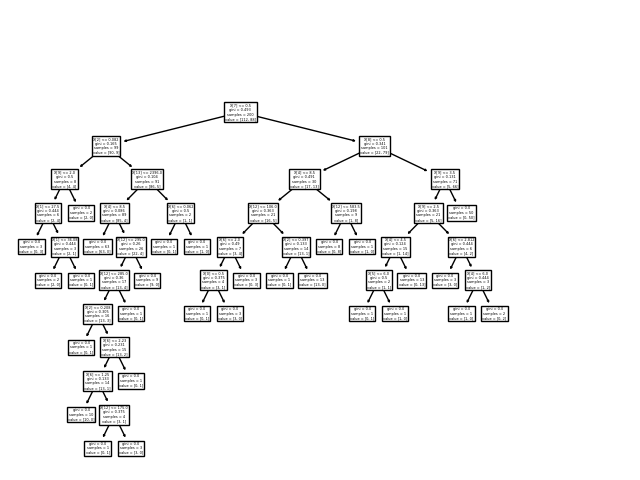
\includegraphics[width=15cm]{images/tree.jpg}
    \caption{Resulting tree for \textit{australian.txt} data (690 samples), Partition with a training set of 200 samples. Maximum depth equal to 20. Testing the decision tree on  the testing dataset (490 samples), the total classification error obtained is equal to 86.}
    \label{fig:1}
\end{figure}
\begin{figure}[H]
    \centering
    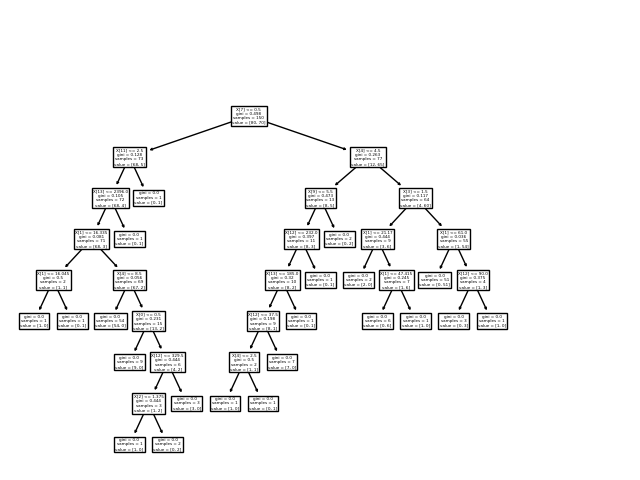
\includegraphics[width=15cm]{images/tree150_113over540.jpg}
    \caption{Resulting tree for \textit{australian.txt} data (690 samples), Partition with a training set of 150 samples. Maximum depth equal to 20. Testing the decision tree on  the testing dataset (540 samples), the total classification error obtained is equal to 113.}
    \label{fig:2}
\end{figure}
\begin{figure}[H]
    \centering
    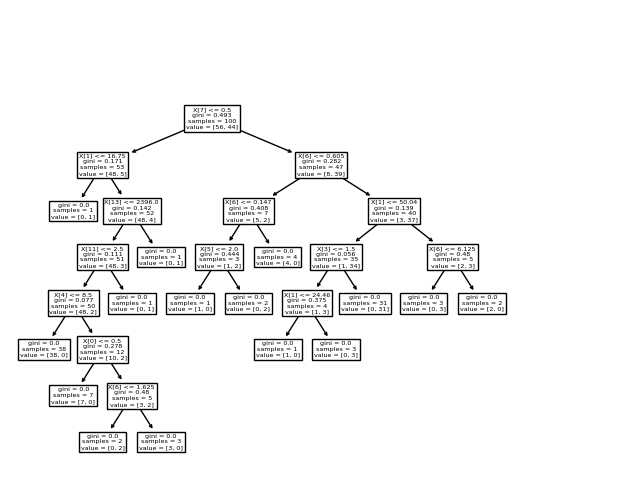
\includegraphics[width=15cm]{images/tree100_171over590.jpg}
    \caption{Resulting tree for \textit{australian.txt} data (690 samples), Partition with a training set of 100 samples. Maximum depth equal to 20. Testing the decision tree on  the testing dataset (590 samples), the total classification error obtained is equal to 171.}
    \label{fig:3}
\end{figure}
\begin{figure}[H]
    \centering
    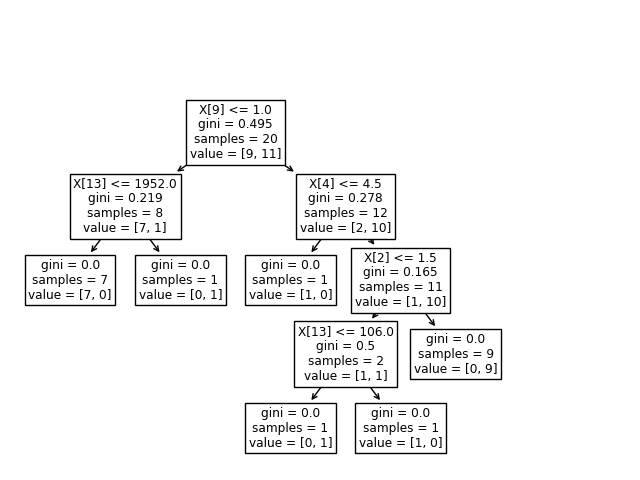
\includegraphics[width=15cm]{images/tree2.jpg}
    \caption{Resulting tree for \textit{australian.txt} data (690 samples), Partition with a training set of 20 samples. Maximum depth equal to 20. Testing the decision tree on  the testing dataset (670 samples), the total classification error obtained is equal to 191.}
    \label{fig:4}
\end{figure}
        
As we can see, these trees are very different from each others. The reason is their different partitions. When the partition has a training set with a low size (i.e. 20 samples, see Figure \ref{fig:4}), then the amount of information used to construct the tree is scarce, and it results in a less accurate (and consequently less deep) tree. When the partition has a training set with a high size (i.e. 200 samples, see Figure \ref{fig:1}), then the amount of information used to construct the tree is higher, and it results in a more accurate (and consequently deeper) tree.

\newpage
\subsection*{Support Vector Machines}
Run SVM to train a classifier, using radial basis as kernel function. Apply cross-validation to evaluate different combinations of values of the model hyper-parameters (box constraint $C$ and kernel parameter $\gamma$). How sensitive is the cross-validation error to changes in $C$ and $\gamma$? Choose the combination of $C$ and $\gamma$ that minimizes the cross-validation error, train the SVM on the entire dataset and report the total classification error.

Advice: use a logarithmic range for $\gamma$.

\begin{figure}[H]
    \begin{subfigure}{0.5\textwidth}
    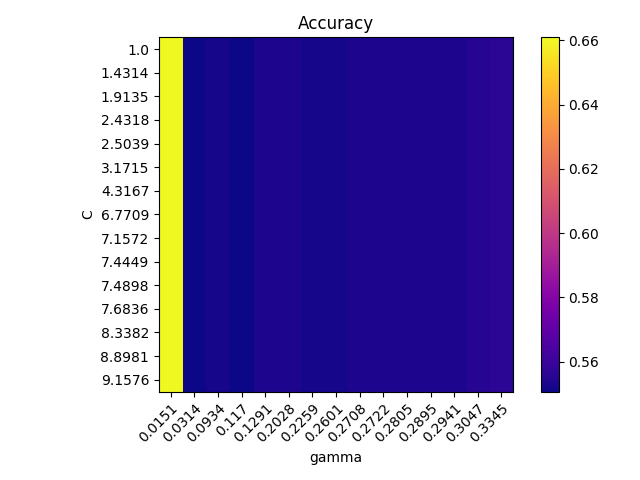
\includegraphics[width=8cm]{images/accuracy_1.jpg} 
    \caption{The mean accuracy on the given test data and labels}
    \label{fig:subfig1}
    \end{subfigure}
    \begin{subfigure}{0.5\textwidth}
    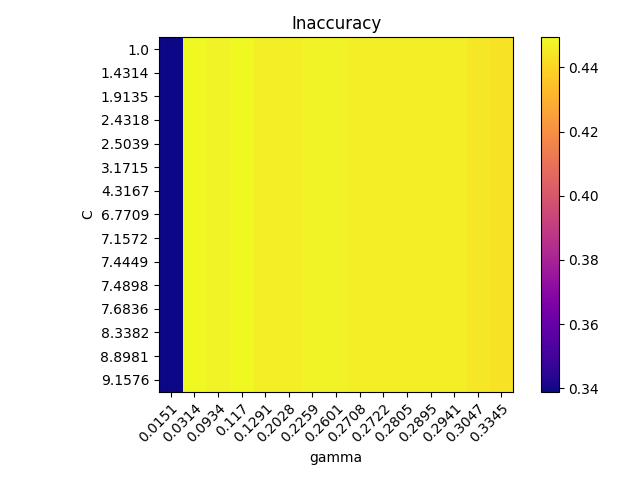
\includegraphics[width=8cm]{images/inaccuracy_1.jpg}
    \caption{The mean inaccuracy on the given test data and labels}
    \label{fig:subfiig2}
    \end{subfigure}
    \caption{Heatmap showing how sensitive is the cross-validation accuracy to changes in $C$ (Y axis) and  $\gamma$ (X axis). Apparently we can interpret that this accuracy is not sensitive to changes in $C$, while it is sensitive to changes in $\gamma$.}
\end{figure}

The minimum of the cross-validation inaccuracy seems to be achieved when $\gamma$ es lower. We plot again this two graphics for lower values of $\gamma$ in order to try to be more accurate.

\begin{figure}[H]
    \begin{subfigure}{0.5\textwidth}
    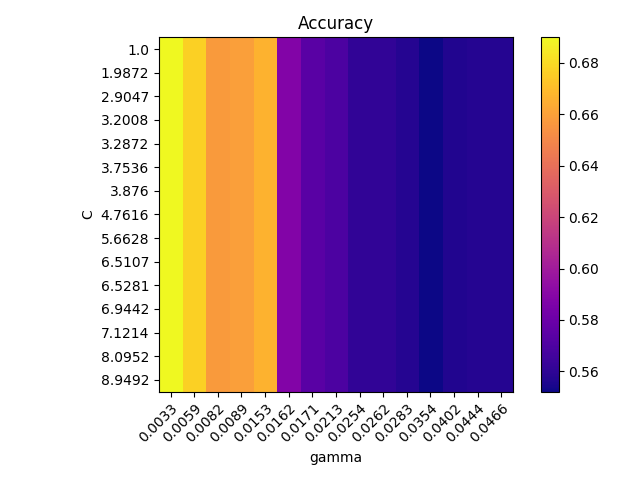
\includegraphics[width=8cm]{images/accuracy_2.jpg} 
    \caption{The mean accuracy on the given test data and labels}
    \label{fig:subfig3}
    \end{subfigure}
    \begin{subfigure}{0.5\textwidth}
    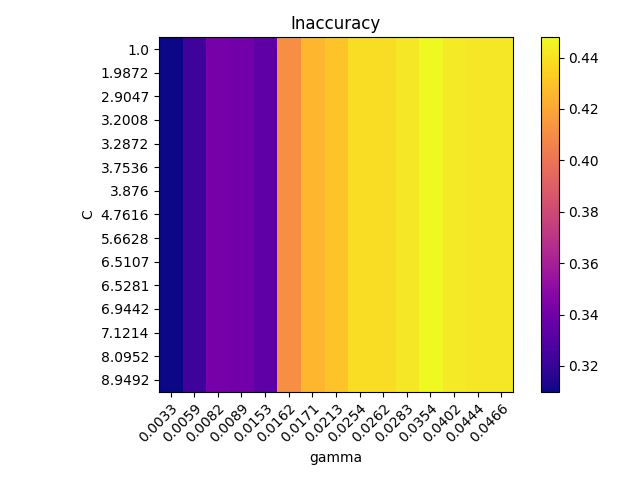
\includegraphics[width=8cm]{images/inaccuracy_2.jpg}
    \caption{The mean inaccuracy on the given test data and labels}
    \label{fig:subfiig4}
    \end{subfigure}
    \caption{Heatmap showing how sensitive is the cross-validation accuracy to changes in $C$ (Y axis) and  lower values of $\gamma$ (X axis). Apparently we can interpret again that this accuracy is not sensitive to changes in $C$, while it is sensitive to changes in $\gamma$.}
\end{figure}

Again, the minimum of the cross-validation inaccuracy seems to be achieved when $\gamma$ even lower. We plot again this two graphics for even lower values of $\gamma$.

\begin{figure}[H]
    \begin{subfigure}{0.5\textwidth}
    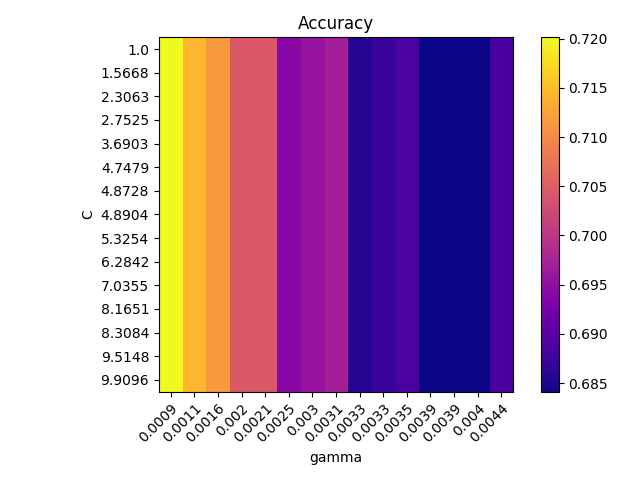
\includegraphics[width=8cm]{images/accuracy_3.jpg} 
    \caption{The mean accuracy on the given test data and labels}
    \label{fig:subfig3}
    \end{subfigure}
    \begin{subfigure}{0.5\textwidth}
    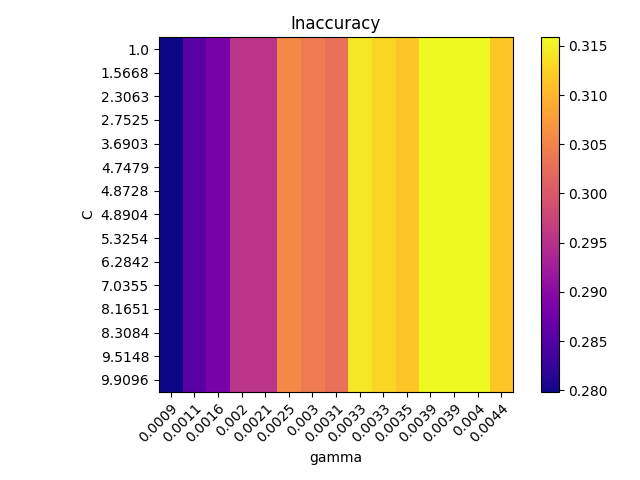
\includegraphics[width=8cm]{images/inaccuracy_3.jpg}
    \caption{The mean inaccuracy on the given test data and labels}
    \label{fig:subfiig4}
    \end{subfigure}
    \caption{Heatmap showing how sensitive is the cross-validation accuracy to changes in $C$ (Y axis) and even lower values of $\gamma$ (X axis). Apparently we can interpret again that this accuracy is not sensitive to changes in $C$, while it is sensitive to changes in $\gamma$.}
\end{figure}

We can finally interpret that the minimum of the cross-validation inaccuracy seems to be achieved when the minimum value of $\gamma$ is achieved, independently from the value of $C$.

\newpage
\subsection*{Neural Networks}
Train a Multi-Layer perceptron using the cross-entropy loss with $\ell-2$ regularization (weight decay penalty). In other words, the activation function equals the logistic function. Plot curves of the training and validation error as a function of the penalty strength $\alpha$. How do the curves behave? Explain why.

Advice: use a logarithmic range for hyper-parameter $\alpha$. Experiment with different sizes of the training/validation sets and different model parameters (network layers).

\begin{figure}[H]
    \begin{subfigure}{0.3\textwidth}
    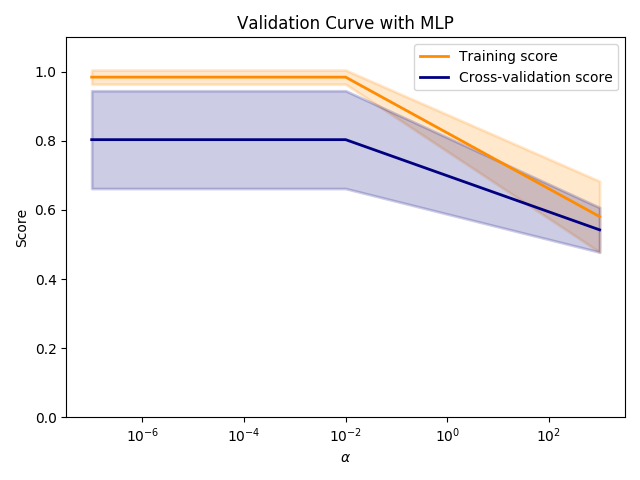
\includegraphics[width=5cm]{images/validationcurve_50.jpg} 
    \caption{Validation curve for a training set of $N=50$}
    \label{fig:subfig5}
    \end{subfigure}
    \begin{subfigure}{0.3\textwidth}
    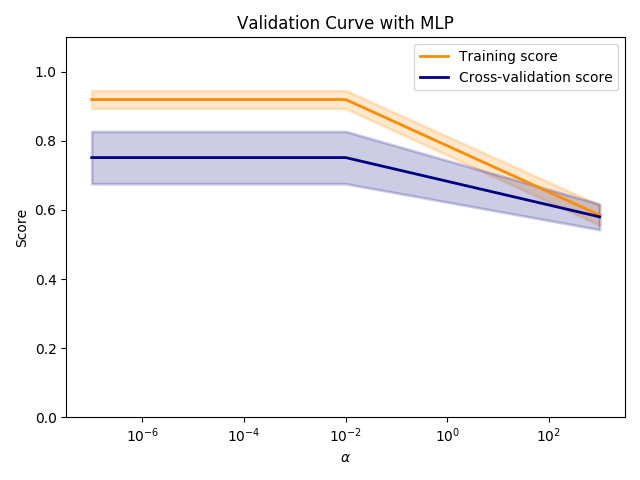
\includegraphics[width=5cm]{images/validationcurve_100.jpg}
    \caption{Validation curve for a training set of $N=100$}
    \label{fig:subfiig6}
    \end{subfigure}
    \begin{subfigure}{0.3\textwidth}
    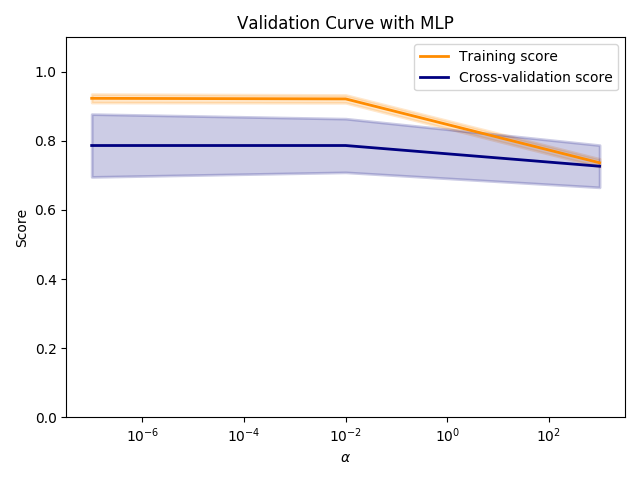
\includegraphics[width=5cm]{images/validationcurve_150.jpg}
    \caption{Validation curve for a training set of $N=150$}
    \label{fig:subfiig7}
    \end{subfigure}
    
    \begin{subfigure}{0.3\textwidth}
    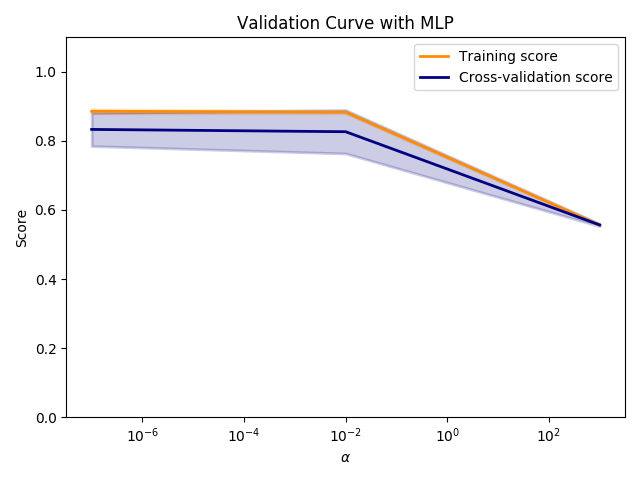
\includegraphics[width=5cm]{images/validationcurve_300.jpg} 
    \caption{Validation curve for a training set of $N=300$}
    \label{fig:subfig5}
    \end{subfigure}
    \begin{subfigure}{0.3\textwidth}
    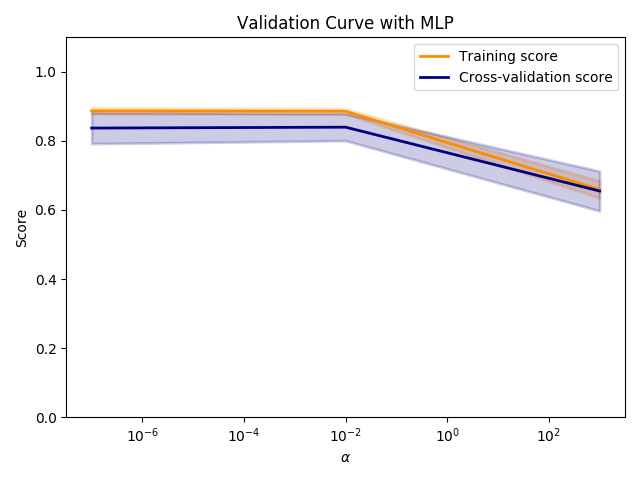
\includegraphics[width=5cm]{images/validationcurve_400.jpg}
    \caption{Validation curve for a training set of $N=400$}
    \label{fig:subfiig6}
    \end{subfigure}
    \begin{subfigure}{0.3\textwidth}
    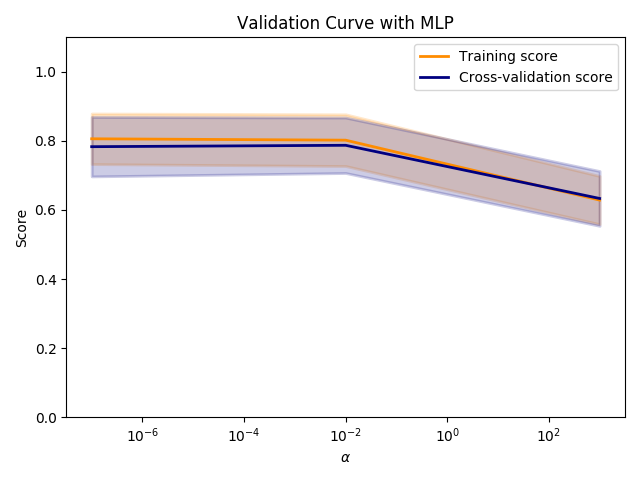
\includegraphics[width=5cm]{images/validationcurve_500.jpg}
    \caption{Validation curve for a training set of $N=500$}
    \label{fig:subfiig7}
    \end{subfigure}
    \caption{Training scores and validation scores of an MLP for different values of the parameter $\alpha$.}
\end{figure}

We know that if the training score and the validation score are both low, the estimator will be underfitting. If the training score is high and the validation score is low, the estimator is overfitting and otherwise it is working very well. We can observe how, increasing the size of the training set, overfitting situation is overcomed. 


\end{document}
